\subsection{Tensorstruktur}

% Definition Masse und Laplace Matrix
\begin{frame}

\begin{framed}
\textbf{Lokale Massenmatrix}
\begin{equation*} \label{eq:mass}
M_{ik} = \int\limits_{T} \varphi_i (\bold{x}) \, \varphi_j (\bold{x}) \, d\bold{x}
\end{equation*}

\textbf{Elementsteifigkeitsmatrix der Laplace Bilinearform}
\begin{equation*}
V_{ij} = \int\limits_{T} \nabla \varphi_i(\bold{x}) \, \nabla \varphi_j(\bold{x})  d \bold{x}
\end{equation*}
\end{framed}

\begin{itemize}
\item $T$ sei die Referenzzelle für Rechtecke
\item $\varphi_i(\bold{x})$ sei eine zweidimensionale reelle Basisfunktion des diskreten Raumes $V_n$ mit $\bold{x}=(x,y)$ .
\end{itemize}

\end{frame}



% Tensorstruktur der Ansatzfunktionen
\begin{frame}
\frametitle{Tensorstruktur der Ansatzfunktionen}

\begin{equation*} \label{eq:tensor}
\varphi^{2D}_i(\bold{x})=\varphi^{2D}_{i_1+(N+1)i_2}(x,y)=\varphi^{1D}_{i_1}(x)\varphi^{1D}_{i_2}(y),
\end{equation*}

\begin{figure}[ht] 
	\centering
  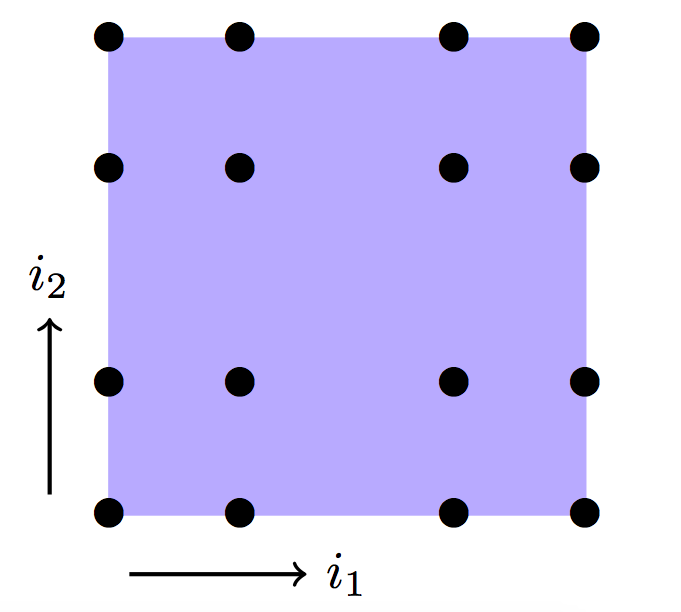
\includegraphics[width=0.3\textwidth]{lexi.png}
	\caption{ \cite[3]{Teachlet}}
	\label{fig:lexi}
\end{figure}

\end{frame}

\begin{frame}
\frametitle{Tensorstruktur der Massenmatrix}
Es seien $\bold{x}_q=(x_{q1},x_{q2})$ die Stützstellen und $\bold{w}_q=w_{q1}w_{q2}$ die Gewichte der Gauss Quadratur.
\begin{equation*} \label{eq:massapprox}
\begin{aligned}
M_{ij} &= \int\limits_{T} \varphi_i (\bold{x}) \, \varphi_j (\bold{x}) \, d\bold{x} \\ \pause
&\approx  \sum\limits_{q=1}^Q \bold{w}_q \, \, \varphi_i (\bold{x}_q) \, \varphi_j (\bold{x}_q) \\ \pause
&= \sum\limits_{q_1=1}^{Q_{1D}} \sum\limits_{q_2=1}^{Q_{1D}} \varphi_{i_1}(x_{q1}) \varphi_{i_2}(x_{q2}) \varphi_{j_1}(x_{q1}) \varphi_{j_2}(x_{q2}) \, w_{q1} w_{q2} \\ 
&= \sum\limits_{q_1=1}^{Q_{1D}} w_{q1} \varphi_{i_1}(x_{q1}) \varphi_{j_1}(x_{q1}) \sum\limits_{q_2=1}^{Q_{1D}} w_{q2} \varphi_{i_2}(x_{q2}) \varphi_{j_2}(x_{q2}) \, . 
\end{aligned}
\end{equation*}
\end{frame}

\begin{frame}
\textbf{Definiere} \\
\begin{itemize}
\item Es sei $\mathcal{N}$ eine Matrix mit $\mathcal{N}_{iq}=\varphi_i(\bold{x}_q)$.
\item Es sei $\mathcal{W}$ eine Matrix mit $\mathcal{W}_{ii}=\bold{w}_i$, sonst Nullen.
\end{itemize}
Dann können wir die Massenmatrix schreiben als
\begin{equation*}
M = \underbrace{\mathcal{N} \mathcal{W}}_{:=\mathcal{W}_N} \mathcal{N}^T. = \mathcal{W}_N \mathcal{N}^T
\end{equation*}
\pause
\textbf{Nutze Tensorstruktur der Ansatzfunktionen}
\begin{equation*}
\begin{aligned}
\mathcal{N} &= \mathcal{N}^{1D} \otimes \mathcal{N}^{1D} \\
\mathcal{W}_N &= \mathcal{W}_N^{1D} \otimes \mathcal{W}_N^{1D}
\end{aligned}
\end{equation*}
\end{frame}

\begin{frame}
\frametitle{Tensorstruktur der Massenmatrix}
\begin{framed}
\begin{equation*}
\begin{aligned}
M &= \mathcal{W}_N \mathcal{N}^T \\
&= (\mathcal{W}_N^{1D} \otimes \mathcal{W}_N^{1D})(\mathcal{N}^{1D} \otimes \mathcal{N}^{1D})^T \\
&= (\mathcal{W}_N^{1D} \otimes \mathcal{W}_N^{1D})((\mathcal{N}^{1D})^T \otimes (\mathcal{N}^{1D})^T) \\
&= (\mathcal{W}_N^{1D} (\mathcal{N}^{1D})^T) \otimes  (\mathcal{W}_N^{1D} (\mathcal{N}^{1D})^T) 
\end{aligned}
\end{equation*}
\end{framed}

\end{frame}





\begin{frame}
\frametitle{Tensorstruktur der Laplace Bilinearform}

\end{frame}